\section{Redukovani uredjeni binarni dijagrami odlu\v{c}ivanja (ROBDD)}
\label{sec:OBDD}

Uredjeni binarni dijagrami odlu\v{c}ivanja (engl. \emph{Ordered Binary Decision Diagrams}, u daljem tekstu \emph{OBDD}) su BDD u kojima se promenljive uvek testiraju u istom redosledu. OBDD se naziva \emph{redukovano}(engl. \emph{Reduced Ordered Binary Decision Diagrams} \cite{ROBDD}, u daljem tekstu \emph{ROBDD}) ukoliko ima slede\'c{}e osobine:
\begin{itemize}
    \item Neredundantnost - Visoko i nisko podstablo svakog \v{c}vora je razli\v{c}ito.
    \item Jedinstvenost - Ne postoje dva razli\v{c}ita \v{c}vora koja testiraju istu promenljivu, a \v{c}ija su podstabla ista.
\end{itemize}

Kao \v{s}to je pomenuto u poglavlju \ref{sec:BinarnaDrvetaOdlucivanja}, binarna drveta odlu\v{c}ivanja poseduju osobinu kanoni\v{c}nosti. Medjutim, kako postoje razli\v{c}ita BDD koja odgovaraju jednom binarnom drvetu odlu\v{c}ivanja, jasno je da BDD nemaju ovu osobinu. Uprkos tome, zbog svojih lepih i jasno definisanih osobina, ROBDD je takodje kanoni\v{c}no. Pro\v{s}irivanjem definicije kanoni\v{c}nosti na ROBDD, dobijamo tvrdjenje: kanoni\v{c}nost ROBDD zna\v{c}i da za fiksan redosled promenljivih, svaka bulovska funkcija ima jedinstvenu reprezentaciju u vidu ROBDD. Ovo zna\v{c}i da mo\v{z}emo uporediti bulovske funkcije konstrukcijom njihovih ROBDD, a ukoliko su ona jednaka, to garantuje njihovu ekvivalentnost.

ROBDD ima najvi\v{s}e dva lista: 0 i 1. U nastavku \'c{}emo ponekad crtati oba, kako bi se smanjila kompleksnost njhovog grafi\v{c}kog prikaza.



\subsection{Konstrukcija ROBDD}
\label{subsec:ROBDDConstruction}

ROBDD se mo\v{z}e konstruisati na vi\v{s}e na\v{c}ina. U ovom poglavlju \'c{}e najpre \'c{}e biti opisana naivna metoda konstrukcije (videti \ref{subsubsec:naiveROBDDConstruction}), a zatim \'c{}e ukratko biti opisana efikasnija metoda (videti \ref{subsubsec:optimalROBDDConstruction}).


\subsubsection{Naivna konstrukcija ROBDD}
\label{subsubsec:naiveROBDDConstruction}

Najjednostavniji na\v{c}in da se konstrui\v{s}e ROBDD je da se najpre konstrui\v{s}e ekvivalentno uredjeno binarno drvo odlu\v{c}ivanja. Nakon toga se primenjuju slede\'c{}a pravila dokle god ona menjaju postoju\'c{}i dijagram:
\begin{itemize}
    \item Pravilo spajanja - Svaka dva podstabla koja imaju izomorfan BDD se spajaju. U baznom slu\v{c}aju to predstavlja spajanje listova koji imaju iste vrednosti (videti sliku \ref{fig:reductionRule}).
    \item Pravilo eliminacije - Ukoliko su i visoko i nisko pod-drvo ista, bazni \v{c}vor se uklanja (videti sliku \ref{fig:eliminationRule}).
\end{itemize}

\begin{figure}[H]
    \centering
    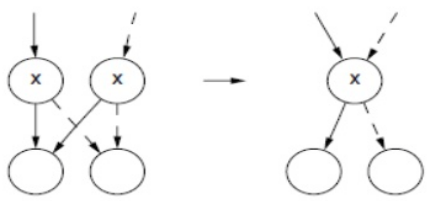
\includegraphics[scale=0.7]{slike/pravilo_spajanja.PNG}
    \caption{Pravilo spajanja}
    \label{fig:reductionRule}
\end{figure}

\begin{figure}[H]
    \centering
    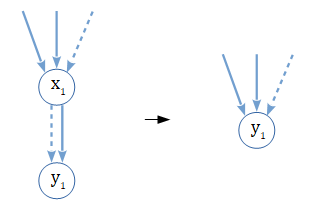
\includegraphics[scale=0.7]{slike/pravilo_eliminacije.PNG}
    \caption{Pravilo eliminacije}
    \label{fig:eliminationRule}
\end{figure}

Mana naivnog pristupa konstrukciji ROBDD je \v{s}to je on uvek eksponencijalne slo\v{z}enosti. Razlog za to je \v{s}to je kostrukcija kompletnog binarnog drveta odlu\v{c}ivanja skupa operacija, koja, pored velike vremenske slo\v{z}enosti, zauzima i eksponencijalno veliku koli\v{c}inu memorije u odnosu na broj promenljivih u ulaznoj formuli.

\begin{exmp}
    Posmatrajmo funkciju
    $$(x_{1} \vee \overline{x_{2}} \vee \overline{x_{3}}) \wedge (x_{1} \vee \overline{x_{2}} \vee x_{3}) \wedge (x_{1} \vee x_{2} \vee \overline{x_{3}}) \wedge (x_{1} \vee x_{2} \vee x_{3})$$
    Koriste\'c{}i prethodno opisani naivni algoritam, konstruisa\'c{}emo ROBDD za zadatu funkciju.
    Najpre, konstruisa\'c{}emo binarno drvo odlu\v{c}ivanja koje odgovara ovoj funkciji. Ono je prikazano na narednoj slici:
    
    \begin{figure}[H]
        \centering
        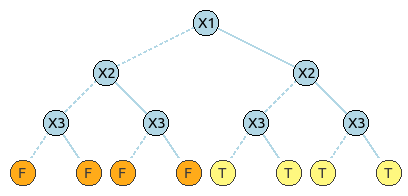
\includegraphics{slike/primer/00.png}
    \end{figure}
    
    Sada po\v{c}injemo da iteriramo dokle god pravila eliminacije ili spajanja imaju efekta.
    
    Pravilom spajanja spajamo prva dva podstabla:
    
    \begin{figure}[H]
        \centering
        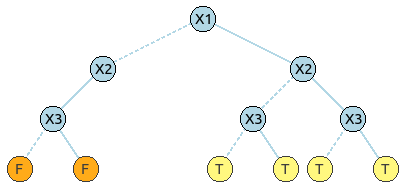
\includegraphics{slike/primer/01.png}
    \end{figure}
    
    Zatim, takodje pravilom spajanja, spajamo dva \emph{F} \v{c}vora.
    
    \begin{figure}[H]
        \centering
        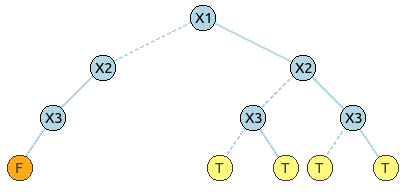
\includegraphics{slike/primer/02.png}
    \end{figure}
    
    Naredna dva koraka su ekvivalentna prethodnim.
    
    \begin{figure}[H]
        \centering
        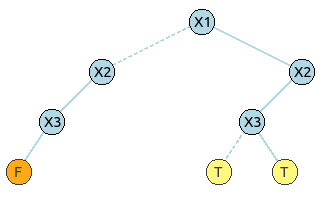
\includegraphics{slike/primer/03.png}
    \end{figure}
    
    \begin{figure}[H]
        \centering
        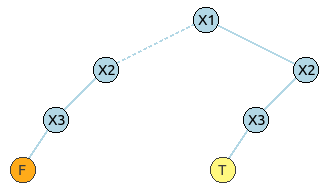
\includegraphics{slike/primer/04.png}
    \end{figure}
    
    U narednom koraku, pravilom eliminacije, bri\v{s}emo \v{c}vor.
    
    \begin{figure}[H]
        \centering
        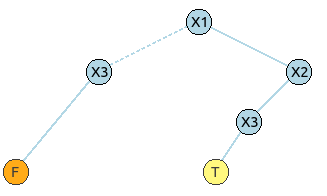
\includegraphics{slike/primer/05.png}
    \end{figure}
    
    Zatim, pravilom eliminacije, bri\v{s}emo naredni \v{c}vor.
    
    \begin{figure}[H]
        \centering
        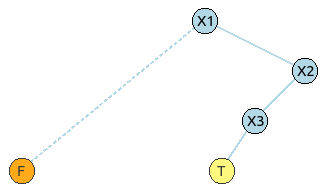
\includegraphics{slike/primer/06.png}
    \end{figure}
    
    Na ekvivalentan na\v{c}in, uklanjamo preostale \v{c}vorove.
    
    \begin{figure}[H]
        \centering
        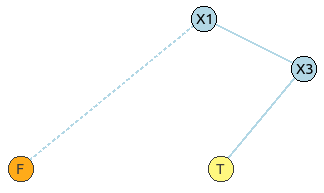
\includegraphics{slike/primer/07.png}
    \end{figure}
        
    \begin{figure}[H]
        \centering
        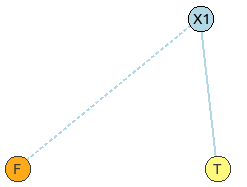
\includegraphics{slike/primer/08.png}
    \end{figure}
    
    Poslednjim korak predstavlja generisani ROBDD. Kao \v{s}to vidimo, ono je zna\v{c}ajno manje od po\v{c}etnog binarnog stabla odlu\v{c}ivanja. Za izra\v{c}unavanje vrednosti funkcije, dovoljno je ispitati samo vrednost promenljive x1.
    
\end{exmp}


\subsubsection{Optimalna konstrukcija ROBDD}
\label{subsubsec:optimalROBDDConstruction}

Drugi na\v{c}in na koji je mogu\'c{}e konstruisati ROBDD takodje ima eksponencijalnu slo\v{z}enost. Medjutim, u praksi on daje dobre rezultate. Za razliku od prethodne metode, preska\v{c}e se medjukorak generisanja binarnog uredjenog drveta odlu\v{c}ivanja. Ovo dovodi do smanjenja potrebne memorije za njegovo generisanje, kao i do zna\v{c}ajnog ubrzanja algoritma.

Postupak je rekurzivan: kre\'c{}e se od bulovske funkcije koja se podeli na podfunkcije za koje se najpre generise ROBDD. Naredni korak je spajanje ove dve funkcije u jednu, uz kori\v{s}\'c{}enje pravila eliminacije i spajanja koja su opisana u prethodnoj sekciji.

Naredni primer oslikava efikasnu metodu za generisanje ROBDD.

\begin{exmp}
    Posmatrajmo funkciju
    $$(x_{1} \vee x_{2}) \wedge (\overline{x_{1}} \vee \overline{x_{2}})$$
    Konstruisa\'c{}emo ROBDD u dva koraka, prvo posmatraju\'c{}i $x_{1} \vee x_{2}$. Iako ve\'c{} znamo kako izgleda ROBDD za ovu funkciju (pogledati poglavlje \ref{sec:BDD}), kako bismo ispo\v{s}tovali postupak idemo dublje i dolazimo do promeljivih $x_{1}$ i $x_{2}$. Njihovi ROBDD su (pritom, redosled smo odabrali tako da $x_{1}$ dolazi pre $x_{2}$):

    \begin{figure}[H]
        \centering
        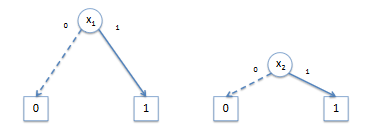
\includegraphics{slike/ROBDD_primer_1.PNG}
    \end{figure}

    Primenjuju\'c{}i bilo koju bulovsku operaciju nad dva ROBDD sa istim redosledom zna\v{c}i krenuto od korena i pratiti paralelne puteve do listova. Kada stignemo do listova, primenjujemo funkciju nad logi\v{c}kom konstantom sadr\v{z}anom u listu kako bismo formirali rezultat za trenutni put. U na\v{s}em primeru, kre\'c{}emo od $x_{1}$ sa levog dijagrama i hipoteti\v{c}kog $x_{1}$ sa desnog dijagrama:

    \begin{figure}[H]
        \centering
        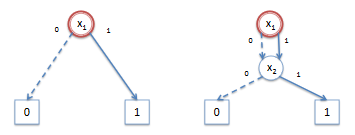
\includegraphics{slike/ROBDD_primer_2.PNG}
    \end{figure}

    Ako pratimo nisku granu sa oba dijagrama, dolazimo do hipoteti\v{c}kog $x_{2}$ na levom dijagramu. Takodje prikazujemo delimi\v{c}no konstruisani rezultuju\'c{}i ROBDD ispod dva ROBDD za promenljive:

    \begin{figure}[H]
        \centering
        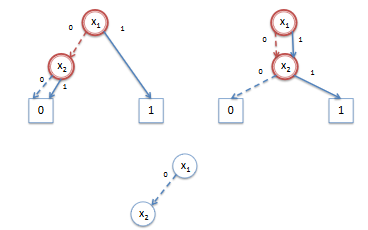
\includegraphics{slike/ROBDD_primer_3.PNG}
    \end{figure}

    S obzirom da niske grane u oba dijagrama vode ka 0, ra\v{c}unamo $0 \vee 0 = 0$ i registrujemo $0$ kao rezultat:

    \begin{figure}[H]
        \centering
        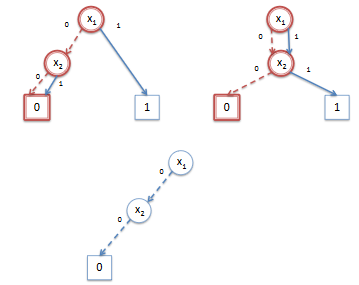
\includegraphics{slike/ROBDD_primer_4.PNG}
    \end{figure}

    Prate\'c{}i visoku granu od $x_{2}$, dolazimo do vrednosti $0$ na levom i $1$ na desnom dijagramu. Primenom funckije dobijamo rezultat $0 \vee 1 = 1$:

    \begin{figure}[H]
        \centering
        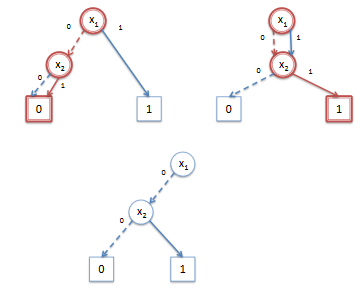
\includegraphics{slike/ROBDD_primer_5.PNG}
    \end{figure}

    Vra\'c{}amo se nazad do $x_{1}$ i razmatramo slu\v{c}aj $x_{1} = 1$ i $x_{2} = 0$. U ovom slu\v{c}aju ra\v{c}unamo $1 \vee 0 = 1$. Napominjemo da je \v{c}vor $x_{2}$ u levom dijagramu samo pomo\'c{} za razumevanje algoritma, u implementaciji se ne bi eksplicitno pravio taj \v{c}vor.

    \begin{figure}[H]
        \centering
        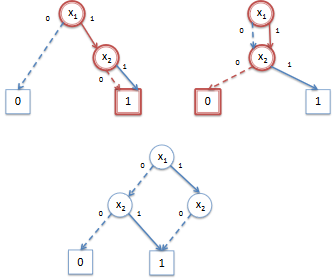
\includegraphics{slike/ROBDD_primer_6.PNG}
    \end{figure}

    Na kraju pratimo visoke grane iz oba $x_{2}$ \v{c}vora i dolazimo do vrednosti $1$:

    \begin{figure}[H]
        \centering
        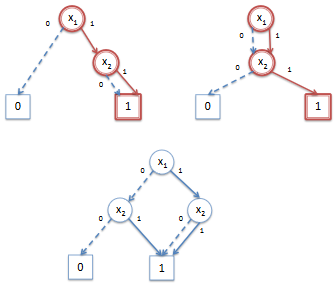
\includegraphics{slike/ROBDD_primer_7.PNG}
    \end{figure}

    Analiziraju\'c{}i rezultat prime\'c{}ujemo da postoje izomorfizmi u konstruisanom dijagramu (pogledati \v{c}vor $x_{2}$ sa desne strane). Stoga, primenjujemo pravilo eliminacije i dobijamo slede\'c{}i rezultat:

    \begin{figure}[H]
        \centering
        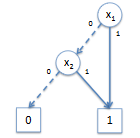
\includegraphics{slike/ROBDD_primer_8.PNG}
    \end{figure}

    ROBDD za funkciju $\overline{x_{1}} \vee \overline{x_{2}}$ se mo\v{z}e dobiti invertovanjem vrednosti u listovima ve\'c{} dobijenog dijagrama. Podsetimo se da smo po\v{c}eli od funkcije $(x_{1} \vee x_{2}) \wedge (\overline{x_{1}} \vee \overline{x_{2}})$ i uspe\v{s}no smo kreirali ROBDD za delove, $(x_{1} \vee x_{2})$ i $(\overline{x_{1}} \vee \overline{x_{2}})$, redom:

    \begin{figure}[H]
        \centering
        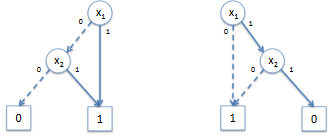
\includegraphics{slike/ROBDD_primer_9.PNG}
    \end{figure}

    Ponavljaju\'c{}i gore opisan postupak za spajanje dijagrama dolazimo do kona\v{c}nog re\v{s}enja:

    \begin{figure}[H]
        \centering
        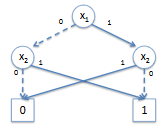
\includegraphics{slike/ROBDD_primer_10.PNG}
    \end{figure}

    Takodje, kako bismo pokazali da se funkcije mogu porediti koriste\'c{}i njihove reprezentacije preko dijagrama (sve dok su te reprezentacije kanoni\v{c}ne), mo\v{z}emo se uveriti da va\v{z}i
    $$(x_{1} \vee x_{2}) \wedge (\overline{x_{1}} \vee \overline{x_{2}}) = x_{1} \oplus x_{2}$$
    jer je gore konstruisani dijagram identi\v{c}an dijagramu za funkciju $\oplus$ (videti sliku \ref{fig:BDOrXor}).
\qed
\end{exmp}
